\section{Map Matching Algorithm}
\subsection{Introduction}
\hspace{2cm} Map-matching algorithms integrate positioning data with spatial road network data (roadway cent relines) to identify  the correct link on which a vehicle is travelling and to determine the location of a vehicle on a link. A map-matching algorithm could be used as a key component to improve the performance of systems that support the navigation function of  intelligent transport systems (ITS). The required horizontal positioning accuracy of such ITS applications is in the range of  1 m to 40 m (95\%) with relatively stringent requirements placed on integrity (quality), continuity and system availability. A  number of map-matching algorithms have been developed by researchers around the world using different techniques such  as topological analysis of spatial road network data, probabilistic theory, Kalman filter, fuzzy logic, and belief theory. The  performances of these algorithms have improved over the years due to the application of advanced techniques in the map  matching processes and improvements in the quality of both positioning and spatial road network data. However, these  algorithms are not always capable of supporting ITS applications with high required navigation performance, especially in  difficult and complex environments such as dense urban areas. This suggests that research should be directed at identifying  any constraints and limitations of existing map matching algorithms as a prerequisite for the formulation of algorithm  improvements.

Map-matching algorithms use inputs generated from positioning technologies (such as GPS) and supplement this with data from a high resolution spatial road network map to provide an enhanced positioning output. The general purpose of a map-matching algorithm is to identify the correct road segment on which the vehicle is travelling and to determine the vehicle location on that segment . Map-matching not only enables the physical location of the vehicle to be identified but also improves the positioning accuracy if good spatial road network data are available. This means that the determination of a vehicle location on a particular road identified by a map-matching algorithm depends to a large extent on the quality of the spatial road map used with the algorithm. A poor
quality road map could lead to a large error in map-matched solutions.
A map-matching algorithm can be developed generically for all applications or for a specific application.\cite{map-matching}

We use topological analysis in our project to define locations of driver (using GPS) .Topology refers to the relationship between entities (points, lines, and polygons). The relationship can be defined as adjacency (in the case of polygons), connectivity (in the case of lines), or containment (in the
case of points in polygons). Therefore, a map-matching algorithm which makes use of the geometry of the
links as well as the connectivity and contiguity of the links is known as a topological map-matching algorithm.We integrate our application with google-map and using distance-matrix service API and using merge sort algorithm to define best driver for our users who request a trip .

\subsection{Google MAP API}

\hspace{2cm} API automatically handles access to Google Maps servers, data downloading, map display, and response to map gestures. You can also use API calls to add markers, polygons, and overlays to a basic map, and to change the user's view of a particular map area. These objects provide additional information for map locations, and allow user interaction with the map. The API allows you to add these graphics to a map:

\begin{itemize}
    
\item Icons anchored to specific positions on the map (Markers).
\item Sets of line segments (Polylines).
\item Enclosed segments (Polygons).
\item Bitmap graphics anchored to specific positions on the map (Ground Overlays).
\item Sets of images which are displayed on top of the base map tiles (Tile Overlays).
\end{itemize} \cite{am004}

We use GeoJSON to identify lines and station locations in project .is an extension of the JSON data format and represents geographical data. Using this utility, you can store geographical features in GeoJSON format and render them as a layer on top of the map. To add and remove your GeoJSON data to and from the map, call addLayerToMap() and removeLayerFromMap() respectively. Similarly you can add and remove individual features by calling addFeature() and removeFeature() and passing in a GeoJsonFeature object. If you want to access the features, you can call getFeatures() to get an iterable of all GeoJsonFeature objects that have been added to the layer.

\textbf{The map object}
\begin{itemize}


The Maps SDK for Android allows you to display a Google map in your Android application. These maps have the same appearance as the maps you see in the Google Maps for Mobile (GMM) app, and the API exposes many of the same features. Two notable differences between the GMM application and the maps displayed by the Maps SDK for Android are:
\begin{itemize}
    \item Map tiles displayed by the API don't contain any personalized content, such as personalized smart icons.
    \item Not all icons on the map are clickable. For example, transit station icons can’t be clicked. However, markers that you add to the map are clickable, and the API has a listener callback interface for various marker interactions.
In addition to mapping functionality, the API also supports a full range of interactions that are consistent with the Android UI model. For example, you can set up interactions with a map by defining listeners that respond to user gestures.
\end{itemize}
The key class when working with a map object is the GoogleMap class. GoogleMap models the map object within your application. Within your UI, a map will be represented by either a MapFragment or MapView object.

GoogleMap handles the following operations automatically:
\begin{itemize}
    \item Connecting to the Google Maps service.
    \item Downloading map tiles.
    \item Displaying tiles on the device screen.
    \item Displaying various controls such as pan and zoom.
    \item Responding to pan and zoom gestures by moving the map and zooming in or out.
\end{itemize}
In addition to these automatic operations, you can control the behavior of maps with objects and methods of the API. For example, GoogleMap has callback methods that respond to keystrokes and touch gestures on the map. You can also set marker icons on your map and add overlays to it, using objects you provide to GoogleMap.
\item \textbf{MapFragment}
MapFragment, a subclass of the Android Fragment class, allows you to place a map in an Android fragment. MapFragment objects act as containers for the map, and provide access to the GoogleMap object.
Unlike a View, a Fragment represents a behavior or a portion of user interface in an activity. You can combine multiple fragments in a single activity to build a multi-pane UI and reuse a fragment in multiple activities. Refer to the Android documentation on Fragments to learn more.

\item\textbf{MapView}

MapView, a subclass of the Android View class, allows you to place a map in an Android View. A View represents a rectangular region of the screen, and is a fundamental building block for Android applications and widgets. Much like a MapFragment, the MapView acts as a container for the map, exposing core map functionality through the GoogleMap object.

When using the API in fully interactive mode, users of the MapView class must forward the following activity lifecycle methods to the corresponding methods in the MapView class: onCreate(), onStart(), onResume(), onPause(), onStop(), onDestroy(), onSaveInstanceState(), and onLowMemory(). The ApiDemos repository on GitHub includes a sample that demonstrates how to forward the activity lifecycle methods. When using the API in lite mode, forwarding lifecycle events is optional.\cite{am004}
\end{itemize}

\textbf{Indoor Maps}

At high zoom levels, the map shows floor plans for indoor spaces such as airports, shopping malls, large retail stores, and transit stations. These floor plans, called indoor maps, are displayed for the 'normal' and 'satellite' map types . They are automatically enabled when the user zooms in, and they fade away when the map is zoomed out.
  Here is a summary of the indoor maps functionality in the API:
\begin{itemize}
    \item You can disable indoor maps by calling GoogleMap.setIndoorEnabled(false). By default, indoor maps are enabled. Indoor maps are displayed on one map at a time. By default this is the first map added to your app. If you'd like to display indoor maps on a different map, disable them on the first map then call setIndoorEnabled(true) on the second map.
\item To disable the default level picker (floor picker), call GoogleMap.getUiSettings().setIndoorLevelPickerEnabled(false). For more details, see Interacting with the Map.

\item An interface on GoogleMap, OnIndoorStateChangeListener, allows you to set a listener to be called when either a new building comes into focus, or a new level is activated in a building. For more details, see Interacting with the Map.
\item GoogleMap.getFocusedBuilding() gives you the building that is currently in focus. You can then find the currently active level by calling IndoorBuilding.getActiveLevelIndex(). Refer to the reference documentation to see all the information available in the IndoorBuilding and IndoorLevel objects.

Styling of the base map does not affect indoor maps.
\end{itemize}


\subsection{Distance Matrix API}
\hspace{2cm} Google's Distance Matrix service computes travel distance and journey duration between multiple origins and destinations using a given mode of travel.

This service does not return detailed route information. Route information, including poly lines and textual directions, can be obtained by passing the desired single origin and destination to the Directions Service.

\textbf{Distance Matrix Requests}
Accessing the Distance Matrix service is asynchronous, since the Google Maps API needs to make a call to an external server. For that reason, you need to pass a callback method to execute upon completion of the request, to process the results.
You access the Distance Matrix service within your code via the google.maps.DistanceMatrixService constructor object. The DistanceMatrixService.getDistanceMatrix() method initiates a request to the Distance Matrix service, passing it a DistanceMatrixRequest object literal containing the origins, destinations, and travel mode, as well as a callback method to execute upon receipt of the response.
\begin{figure}[htp]%
    \centre%
    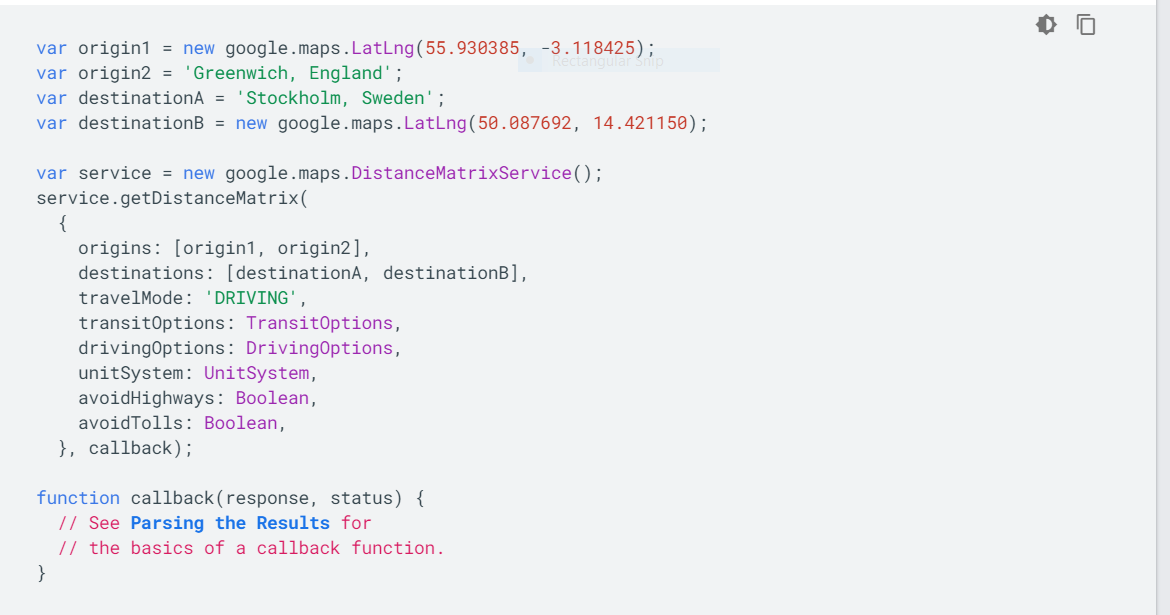
\includegraphics[width=1\textwidth]{images/ch4/request.PNG}%
     % you need to add the caption for the list of figures
    \caption[Example of distance matrix request]{Example of distance matrix request}\label{fig:Example of distance matrix request}%
  \end{figure}
 The DistanceMatrixRequest contains the following fields:
\begin{itemize}
    \item origins (required) — An array containing one or more address strings, google.maps.LatLng objects, or google.maps.Place objects from which to calculate distance and time.
    \item destinations (required) — An array containing one or more address strings, google.maps.LatLng objects, or google.maps.Place objects to which to calculate distance and time.
    \item travelMode (optional) — The mode of transport to use when calculating directions. See the section on travel modes.
    \item  transitOptions (optional) — Options that apply only to requests where travelMode is TRANSIT. Valid values are described in the section on transit options.
    \item drivingOptions (optional) specifies values that apply only to requests where travelMode is DRIVING. Valid values are described in the section on Driving Options.
    \item unitSystem (optional) — The unit system to use when displaying distance. Accepted values are:
    google.maps.UnitSystem.METRIC (default)
    google.maps.UnitSystem.IMPERIAL
    \item avoidHighways (optional) — If true, the routes between origins and destinations will be calculated to avoid highways where possible.
    \item avoidTolls (optional) — If true, the directions between points will be calculated using non-toll routes, wherever possible.\cite{am005}
\end{itemize}

\subsection{Merge Sort}
\hspace{2cm} We can obtain the list addresses of available drivers and there are available seats on them cars by using distance matrix API . We use merge sort to obtain nearest driver from user's location and match between them .

\textbf{Merge sort works as follows: }
\begin{enumerate}
     \item Divide the unsorted list into n sublists, each containing one element (a list of one element is considered sorted).
    \item Repeatedly merge sublists to produce new sorted sublists until there is only one sublist remaining. This will be the sorted list.
\end{enumerate}

Example of Merge Sort in detail\cite{am007} :
\begin{enumerate}
    \item  We take an unsorted array as the following 
 \begin{figure}[htp]%
    \centre%
    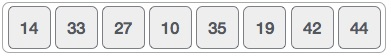
\includegraphics[width=0.1\textwidth]{images/ch4/unsorted_array.jpg}%
     % you need to add the caption for the list of figures
    \caption[unsorted array]{unsorted array}\label{fig:unsorted array}%
  \end{figure}

\item We know that merge sort first divides the whole array iterative into equal halves unless the atomic values are achieved. We see here that an array of 8 items is divided into two arrays of size 4.
\begin{figure}[htp]%
    \centre%
    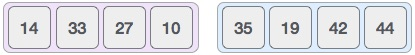
\includegraphics[width=1\textwidth]{images/ch4/merge_sort_divide_1.jpg}%
     % you need to add the caption for the list of figures
    \caption[Merge Sort divide-1]{Divide-1}\label{fig:divide}%
  \end{figure}
  
\item This does not change the sequence of appearance of items in the original. Now we divide these two arrays into halves.
\begin{figure}[htp]%
    \centre%
    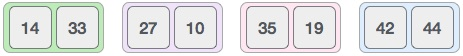
\includegraphics[width=1\textwidth]{images/ch4/merge_sort_divide_2.jpg}%
     % you need to add the caption for the list of figures
    \caption[Merge Sort divide-1]{Divide-2}\label{fig:Integration with google-map}%
  \end{figure}

\item We further divide these arrays and we achieve atomic value which can no more be divided.
\begin{figure}[htp]%
    \centre%
    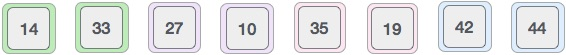
\includegraphics[width=1\textwidth]{images/ch4/merge_sort_divide_3.jpg}%
     % you need to add the caption for the list of figures
    \caption[Merge Sort divide-3]{Divide-3}\label{fig:Integration with google-map}%
  \end{figure}

\item Now, we combine them in exactly the same manner as they were broken down. Please note the color codes given to these lists.

We first compare the element for each list and then combine them into another list in a sorted manner. We see that 14 and 33 are in sorted positions. We compare 27 and 10 and in the target list of 2 values we put 10 first, followed by 27. We change the order of 19 and 35 whereas 42 and 44 are placed sequentially.
\begin{figure}[htp]%
    \centre%
    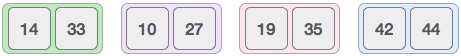
\includegraphics[width=1\textwidth]{images/ch4/merge_sort_combine_1.jpg}%
     % you need to add the caption for the list of figures
    \caption[Merge Sort combine-1]{Combine-1}\label{fig:Combine-1}%
  \end{figure}
  
\item In the next iteration of the combining phase, we compare lists of two data values, and merge them into a list of found data values placing all in a sorted order.\newline

\begin{figure}[htp]%
    \centre%
    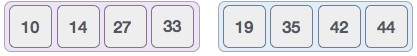
\includegraphics[width=1\textwidth]{images/ch4/merge_sort_combine_2.jpg}%
     % you need to add the caption for the list of figures
    \caption[Merge Sort combine-2]{Combine-2}\label{fig:Combine-2}%
  \end{figure}
  \newline
\item After the final merging, the list should look like this
\newline
    \begin{figure}[htp]%
    \centre%
    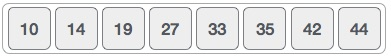
\includegraphics[width=1\textwidth]{images/ch4/merge_sort.jpg}%
     % you need to add the caption for the list of figures
    \caption[Sorted array after merge sort]{Sorted array by Merge Sort}\label{fig:Sorted array}%
    \end{figure}
    \end{enumerate}
  Merge sort is a sorting technique based on divide and conquer technique. With worst-case time complexity being Ο(n log n), it is one of the most respected algorithms.\cite{am007}
